\documentclass[border=5pt]{standalone}
\usepackage{tikz}
\usepackage{amsmath}
\usetikzlibrary{calc, positioning, arrows.meta, 3d}
\begin{document}
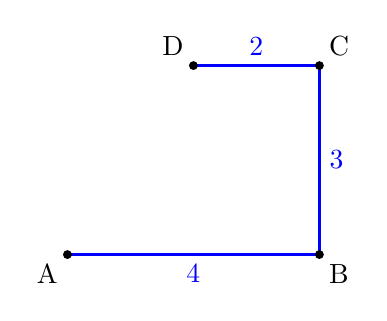
\begin{tikzpicture}[scale=0.8]
% Draw the wire segments
\draw[thick, blue] (0,0) -- (4,0) node[midway, below] {4};
\draw[thick, blue] (4,0) -- (4,3) node[midway, right] {3};
\draw[thick, blue] (4,3) -- (2,3) node[midway, above] {2};

% Mark points
\fill (0,0) circle (2pt) node[below left] {A};
\fill (4,0) circle (2pt) node[below right] {B};
\fill (4,3) circle (2pt) node[above right] {C};
\fill (2,3) circle (2pt) node[above left] {D};
\end{tikzpicture}
\end{document}
